\documentclass{article}
\usepackage[scaled]{helvet}
\renewcommand\familydefault{\sfdefault}
\usepackage[T1]{fontenc}
\usepackage{fancyhdr}
\usepackage{graphicx}
\usepackage{subfigure}
\usepackage{booktabs}
\usepackage[inline]{enumitem}
\usepackage{amsmath}
\usepackage{hyperref}
\hypersetup{
    colorlinks=true,
    citecolor=[RGB]{0,0.5,0.5},
    urlcolor=[RGB]{0,0.5,0.5},
    linkcolor=[RGB]{0,0.5,0.5}
}
\usepackage{geometry}
\geometry{margin={0.8in,1in}}
\title{CMPT 423-820 Mini Project 3 Report}
\author{Corbin Knipfel \and David Simonov \and Sadi Mohammad Mustafa \and Sadman Iqbal}
\date{}
\begin{document}
\maketitle
\hrule
\vspace{0.2in}
\section{Distortion vs K}
\begin{figure}[ht]
    \centering
    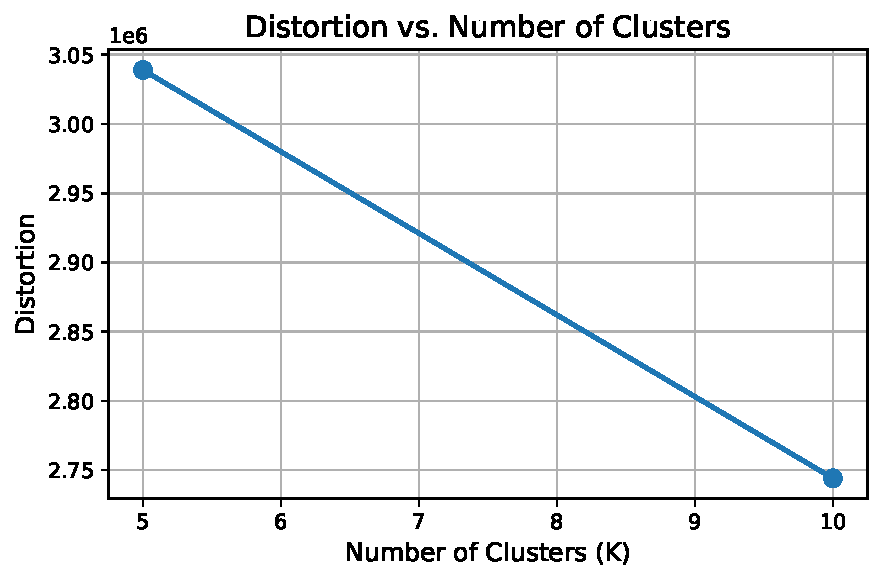
\includegraphics[width=0.8\linewidth]{figures/distortion_plot.pdf}
    \caption{Distortion as a function of the number of clusters \(K\).}
    \label{fig:distortion}
\end{figure}
\noindent
\textbf{Description:} \\
The graph illustrates how distortion decreases as the number of clusters (K) increases from 5 to 10. This follows the expected pattern for K-means clustering, where higher values of K lead to lower distortion as data points can be assigned to more specific centroids. The distortion is defined as $J(\mu_1, ...,\mu_k;Z) = \sum_{i=1}^{N} \|x_i - \sum_{k=1}^{K} z_{i,k}\mu_k\|^2$, which measures the sum of squared distances between each data point and its assigned centroid. The notable reduction in distortion from K=5 to K=10 suggests that the MNIST dataset benefits from having a larger number of clusters, aligning with the intuition that there are 10 distinct digit classes in the data.
\vspace{1.5em}
\section{Cluster Centroid Visualizations}
\subsection*{Centroids for Lowest K Value}
\begin{figure}[ht]
    \centering
    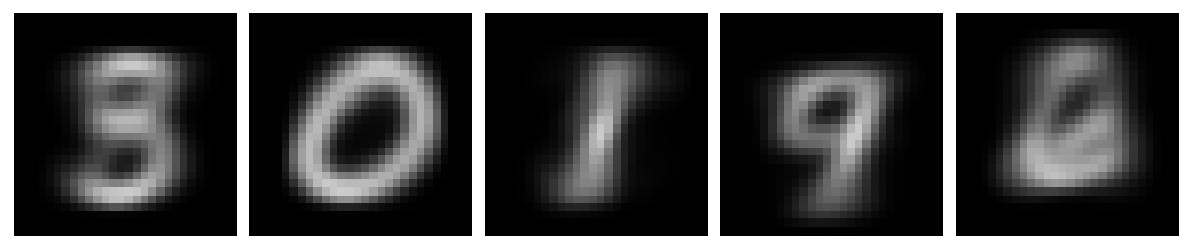
\includegraphics[width=0.8\linewidth]{figures/centroids_k5.pdf}
    \caption{Cluster centroids for \(K = 5\).}
    \label{fig:centroids_k5}
\end{figure}
\noindent
\textbf{Description:} \\
With K=5, the centroids show broader, more general patterns that combine features from multiple digit classes. Each centroid represents an average of several digit types that share similar visual characteristics. For example, one centroid might capture digits with strong vertical strokes (like 1, 4, and 7), while another might represent digits with more rounded features (like 0, 6, and 8). The centroids appear blurred because they are attempting to represent multiple distinct digit classes simultaneously. This visualization demonstrates that K=5 is insufficient to properly separate all ten digit classes in the MNIST dataset, as each centroid must represent approximately two digit classes on average.
\vspace{1.5em}
\subsection*{Centroids for Highest K Value}
\begin{figure}[ht]
    \centering
    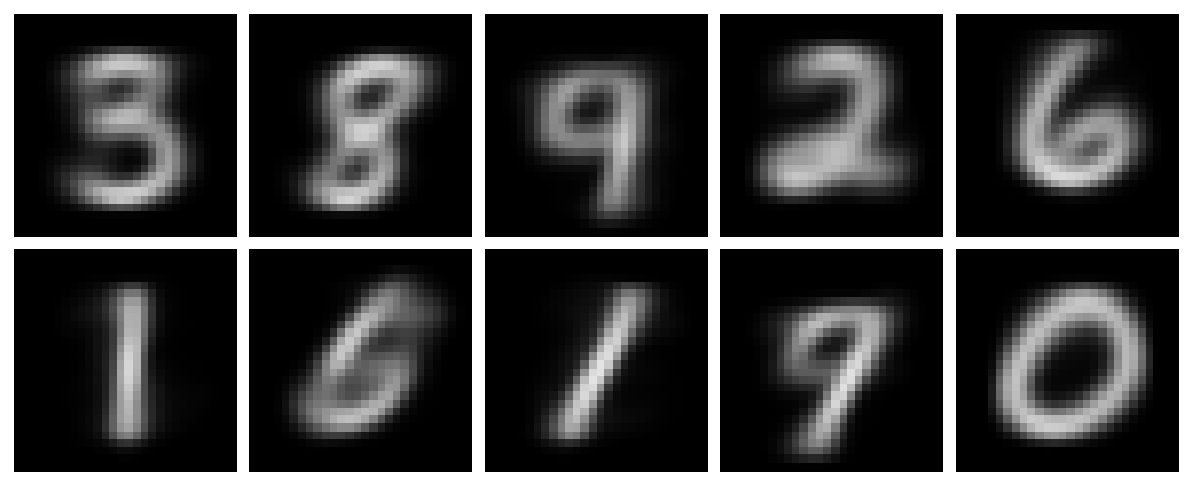
\includegraphics[width=0.8\linewidth]{figures/centroids_k10.pdf}
    \caption{Cluster centroids for \(K = 10\).}
    \label{fig:centroids_k10}
\end{figure}
\noindent
\textbf{Description:} \\
With K=10, the centroids display much clearer, more distinct patterns that closely resemble individual digit classes. Each centroid has captured characteristics specific to a particular digit, showing more defined shapes compared to the K=5 case. The sharper features in these centroids indicate that K=10 allows the algorithm to more effectively separate the different digit classes in the feature space. However, the correspondence between centroids and actual digit classes may not be perfect, some digits with similar visual features might still influence each other's centroids, while digits with high variance in writing styles might be represented by centroids that don't clearly resemble canonical versions of those digits.
\vspace{1.5em}
\section{Discussion: Can K-Means Find 10 Digit Classes?}
\noindent
K-means clustering demonstrates varying effectiveness in identifying the 10 digit classes in the MNIST dataset. When K=10, there is a natural correspondence we might expect between the number of clusters and the number of digit classes. Our analysis shows that K-means does capture meaningful patterns that align with the digit classes, but with several limitations.

First, K-means clustering using Euclidean distance in pixel space doesn't always align with perceptual similarity. Digits that appear visually similar in their pixel representation (like 5 and 8, or 1 and 7) might be confused or placed in clusters that don't precisely match their semantic classes. This is evident in our centroid visualizations, where some clusters contain mixed features from multiple digits.

Second, the random initialization of centroids can lead to suboptimal clustering. Despite running multiple repeats and choosing the best result based on distortion, there's no guarantee that the algorithm will find clusters that perfectly align with the digit classes. Some runs might split a single digit class across multiple clusters or combine different digit classes into one cluster.

Third, K-means assumes spherical clusters of similar sizes, but the natural distribution of handwritten digits in feature space may not conform to this assumption. Some digit classes exhibit higher variance in writing styles (e.g., the digit 7 is often written with or without a horizontal stroke), potentially leading to a single digit being split across multiple clusters.

Despite these limitations, our experiments with K=10 show that K-means can capture a significant portion of the natural class structure in the MNIST dataset. The centroids reveal patterns that are recognizable as digits, suggesting that unsupervised K-means clustering can discover meaningful structure in the data without using label information. In applications where labeled data is unavailable or expensive to obtain, K-means could serve as a useful preprocessing step or as a way to gain initial insights into the structure of image data.
\end{document}